% Generated by extension/synthesis/make_assets.py. Do not edit.
\definecolor{propcol}{HTML}{217D91}
\definecolor{pairedcol}{HTML}{5D6670}
\definecolor{semicol}{HTML}{C9803A}
\definecolor{champcol}{HTML}{8E4B8C}
\definecolor{ridgecol}{HTML}{9AA3AB}
\definecolor{meancol}{HTML}{A64442}
\definecolor{sitecol}{HTML}{6A8FB3}
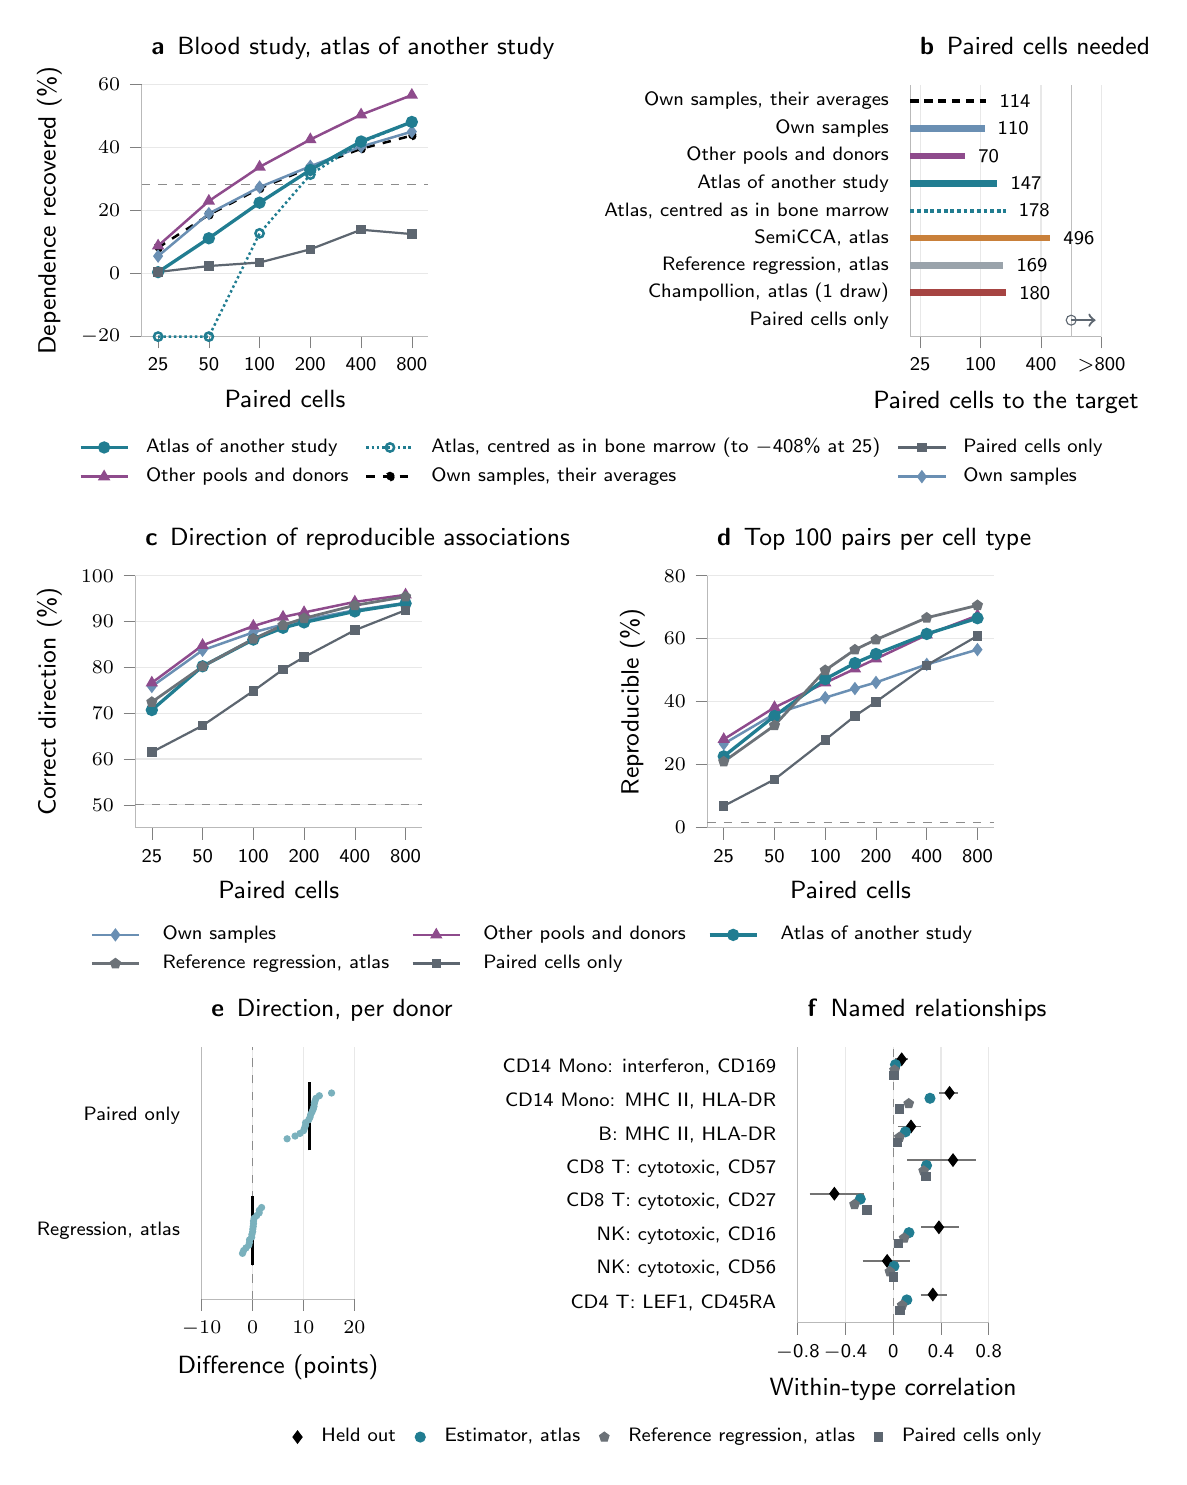
\begin{tikzpicture}[font=\sffamily]
\begin{axis}[name=a,scale only axis,width=.3\textwidth,height=3.2cm,xmode=log,log basis x=2,
 xmin=20,xmax=1000,ymin=-20,ymax=60,xtick={25,50,100,200,400,800},xticklabels={25,50,100,200,400,800},ytick={-20,0,20,40,60},
 xlabel={Paired cells},ylabel={Dependence recovered (\%)},
 title={\textbf{a}\enspace Blood study, atlas of another study},
 axis x line*=bottom,axis y line*=left,tick align=outside,ymajorgrids=true,grid style={gray!18},axis line style={gray!55},tick label style={font=\sffamily\scriptsize},label style={font=\sffamily\small},clip=false,title style={font=\sffamily\small,at={(0,1)},anchor=base west,yshift=5pt}]
\draw[dashed,black!45] (axis cs:20,28.34) -- (axis cs:1000,28.34);
\addplot[color=black,line width=.9pt,dashed,mark=*,mark size=1.3pt] coordinates { (25,8.22) (50,18.67) (100,27.05) (200,33.65) (400,39.65) (800,43.83) };
\addplot[color=sitecol,line width=.9pt,mark=diamond*,mark size=1.7pt] coordinates { (25,5.56) (50,19.06) (100,27.46) (200,34.07) (400,40.31) (800,45.08) };
\addplot[color=champcol,line width=.9pt,mark=triangle*,mark size=1.7pt] coordinates { (25,8.83) (50,23.04) (100,33.86) (200,42.57) (400,50.44) (800,56.67) };
\addplot[color=propcol,line width=1.2pt,mark=*,mark size=1.6pt] coordinates { (25,0.46) (50,11.22) (100,22.52) (200,32.92) (400,41.95) (800,48.15) };
\addplot[color=propcol,line width=.9pt,densely dotted,mark=o,mark size=1.5pt,mark options={solid}] coordinates { (25,-20.00) (50,-20.00) (100,12.78) (200,31.44) (400,41.69) (800,48.09) };
\addplot[color=pairedcol,line width=.8pt,mark=square*,mark size=1.3pt] coordinates { (25,0.52) (50,2.41) (100,3.52) (200,7.72) (400,13.93) (800,12.55) };
\end{axis}
\begin{axis}[at={(a.outer north east)},anchor=outer north west,xshift=.4cm,name=b,scale only axis,width=.2\textwidth,height=3.2cm,xmode=log,log basis x=2,
 xmin=20,xmax=1600,ymin=.4,ymax=9.6,xtick={25,100,400,1600},xticklabels={25,100,400,$>$800},
 ytick={1,2,3,4,5,6,7,8,9},
 yticklabels={{Paired cells only},{Champollion, atlas (1 draw)},{Reference regression, atlas},{SemiCCA, atlas},{Atlas, centred as in bone marrow},{Atlas of another study},{Other pools and donors},{Own samples},{Own samples, their averages}},
 xlabel={Paired cells to the target},
 title={\textbf{b}\enspace Paired cells needed},
 axis x line*=bottom,axis y line*=left,tick align=outside,xmajorgrids=true,grid style={gray!18},axis line style={gray!55},tick label style={font=\sffamily\scriptsize},label style={font=\sffamily\small},clip=false,title style={font=\sffamily\small,at={(0,1)},anchor=base west,yshift=5pt},y tick style={draw=none}]
\draw[black!25] (axis cs:800,.4) -- (axis cs:800,9.6);
\draw[->,color=pairedcol,line width=.8pt] (axis cs:800,1) -- (axis cs:1400,1);
\addplot[only marks,mark=o,mark size=1.8pt,color=pairedcol] coordinates { (800,1) };
\draw[color=meancol,line width=2.4pt] (axis cs:20,2) -- (axis cs:180.0,2);
\node[font=\sffamily\scriptsize,anchor=west] at (axis cs:194.4,2) {180};
\draw[color=ridgecol,line width=2.4pt] (axis cs:20,3) -- (axis cs:168.9,3);
\node[font=\sffamily\scriptsize,anchor=west] at (axis cs:182.4,3) {169};
\draw[color=semicol,line width=2.4pt] (axis cs:20,4) -- (axis cs:495.7,4);
\node[font=\sffamily\scriptsize,anchor=west] at (axis cs:535.4,4) {496};
\draw[color=propcol,line width=1.4pt,densely dotted] (axis cs:20,5) -- (axis cs:178.2,5);
\node[font=\sffamily\scriptsize,anchor=west] at (axis cs:192.5,5) {178};
\draw[color=propcol,line width=2.4pt] (axis cs:20,6) -- (axis cs:147.3,6);
\node[font=\sffamily\scriptsize,anchor=west] at (axis cs:159.1,6) {147};
\draw[color=champcol,line width=2.4pt] (axis cs:20,7) -- (axis cs:70.2,7);
\node[font=\sffamily\scriptsize,anchor=west] at (axis cs:75.8,7) {70};
\draw[color=sitecol,line width=2.4pt] (axis cs:20,8) -- (axis cs:109.6,8);
\node[font=\sffamily\scriptsize,anchor=west] at (axis cs:118.4,8) {110};
\draw[color=black,line width=1.6pt,densely dashed] (axis cs:20,9) -- (axis cs:114.5,9);
\node[font=\sffamily\scriptsize,anchor=west] at (axis cs:123.7,9) {114};
\end{axis}
\path (a.outer south west) -- (b.outer south east) coordinate[pos=.5] (legab);
\begin{axis}[hide axis,scale only axis,width=1pt,height=1pt,xmin=0,xmax=1,ymin=0,ymax=1,at={(legab)},anchor=north,yshift=-2pt,legend style={draw=none,font=\sffamily\scriptsize,at={(0.5,0.5)},anchor=north,legend columns=3,column sep=4pt,cells={anchor=west}}]
\addlegendimage{color=propcol,line width=1.2pt,mark=*,mark size=1.6pt}
\addlegendentry{Atlas of another study}
\addlegendimage{color=propcol,line width=.9pt,densely dotted,mark=o,mark size=1.5pt,mark options={solid}}
\addlegendentry{Atlas, centred as in bone marrow (to \ensuremath{-}408\% at 25)}
\addlegendimage{color=pairedcol,line width=.8pt,mark=square*,mark size=1.3pt}
\addlegendentry{Paired cells only}
\addlegendimage{color=champcol,line width=.9pt,mark=triangle*,mark size=1.7pt}
\addlegendentry{Other pools and donors}
\addlegendimage{color=black,line width=.9pt,dashed,mark=*,mark size=1.3pt}
\addlegendentry{Own samples, their averages}
\addlegendimage{color=sitecol,line width=.9pt,mark=diamond*,mark size=1.7pt}
\addlegendentry{Own samples}
\end{axis}
\begin{axis}[at={(a.outer south west)},anchor=outer north west,yshift=-1.3cm,name=c,scale only axis,width=.3\textwidth,height=3.2cm,xmode=log,log basis x=2,
 xmin=20,xmax=1000,ymin=45,ymax=100,xtick={25,50,100,200,400,800},xticklabels={25,50,100,200,400,800},ytick={50,60,70,80,90,100},
 xlabel={Paired cells},ylabel={Correct direction (\%)},
 title={\textbf{c}\enspace Direction of reproducible associations},
 axis x line*=bottom,axis y line*=left,tick align=outside,ymajorgrids=true,grid style={gray!18},axis line style={gray!55},tick label style={font=\sffamily\scriptsize},label style={font=\sffamily\small},clip=false,title style={font=\sffamily\small,at={(0,1)},anchor=base west,yshift=5pt}]
\draw[dashed,black!45] (axis cs:20,50.000) -- (axis cs:1000,50.000);
\addplot[color=sitecol,line width=.9pt,mark=diamond*,mark size=1.7pt] coordinates { (25,75.83) (50,83.74) (100,87.65) (150,89.36) (200,90.33) (400,92.47) (800,94.07) };
\addplot[color=champcol,line width=.9pt,mark=triangle*,mark size=1.7pt] coordinates { (25,76.63) (50,84.82) (100,89.01) (150,90.99) (200,91.99) (400,94.29) (800,95.83) };
\addplot[color=propcol,line width=1.2pt,mark=*,mark size=1.6pt] coordinates { (25,70.69) (50,80.24) (100,86.07) (150,88.64) (200,89.82) (400,92.22) (800,93.95) };
\addplot[color=pairedcol,line width=.8pt,mark=square*,mark size=1.3pt] coordinates { (25,61.50) (50,67.29) (100,74.85) (150,79.54) (200,82.25) (400,88.12) (800,92.48) };
\addplot[color=ridgecol!70!black,line width=1pt,mark=pentagon*,mark size=1.5pt] coordinates { (25,72.43) (50,80.20) (100,86.22) (150,89.20) (200,90.72) (400,93.54) (800,95.42) };
\end{axis}
\begin{axis}[at={(c.outer north east)},anchor=outer north west,xshift=.4cm,name=d,scale only axis,width=.3\textwidth,height=3.2cm,xmode=log,log basis x=2,
 xmin=20,xmax=1000,ymin=0,ymax=80,xtick={25,50,100,200,400,800},xticklabels={25,50,100,200,400,800},ytick={0,20,40,60,80},
 xlabel={Paired cells},ylabel={Reproducible (\%)},
 title={\textbf{d}\enspace Top 100 pairs per cell type},
 axis x line*=bottom,axis y line*=left,tick align=outside,ymajorgrids=true,grid style={gray!18},axis line style={gray!55},tick label style={font=\sffamily\scriptsize},label style={font=\sffamily\small},clip=false,title style={font=\sffamily\small,at={(0,1)},anchor=base west,yshift=5pt}]
\draw[dashed,black!45] (axis cs:20,1.598) -- (axis cs:1000,1.598);
\addplot[color=sitecol,line width=.9pt,mark=diamond*,mark size=1.7pt] coordinates { (25,26.63) (50,36.13) (100,41.30) (150,44.19) (200,46.12) (400,51.86) (800,56.55) };
\addplot[color=champcol,line width=.9pt,mark=triangle*,mark size=1.7pt] coordinates { (25,28.07) (50,38.18) (100,46.00) (150,50.47) (200,53.63) (400,61.23) (800,67.37) };
\addplot[color=propcol,line width=1.2pt,mark=*,mark size=1.6pt] coordinates { (25,22.66) (50,35.46) (100,47.19) (150,52.26) (200,55.16) (400,61.53) (800,66.52) };
\addplot[color=pairedcol,line width=.8pt,mark=square*,mark size=1.3pt] coordinates { (25,6.91) (50,15.33) (100,27.90) (150,35.47) (200,39.98) (400,51.59) (800,60.91) };
\addplot[color=ridgecol!70!black,line width=1pt,mark=pentagon*,mark size=1.5pt] coordinates { (25,20.98) (50,32.47) (100,49.99) (150,56.52) (200,59.71) (400,66.66) (800,70.61) };
\end{axis}
\path (c.outer south west) -- (d.outer south east) coordinate[pos=.5] (legcd);
\begin{axis}[hide axis,scale only axis,width=1pt,height=1pt,xmin=0,xmax=1,ymin=0,ymax=1,at={(legcd)},anchor=north,yshift=-2pt,legend style={draw=none,font=\sffamily\scriptsize,at={(0.5,0.5)},anchor=north,legend columns=3,column sep=6pt,cells={anchor=west}}]
\addlegendimage{color=sitecol,line width=.9pt,mark=diamond*,mark size=1.7pt}
\addlegendentry{Own samples}
\addlegendimage{color=champcol,line width=.9pt,mark=triangle*,mark size=1.7pt}
\addlegendentry{Other pools and donors}
\addlegendimage{color=propcol,line width=1.2pt,mark=*,mark size=1.6pt}
\addlegendentry{Atlas of another study}
\addlegendimage{color=ridgecol!70!black,line width=1pt,mark=pentagon*,mark size=1.5pt}
\addlegendentry{Reference regression, atlas}
\addlegendimage{color=pairedcol,line width=.8pt,mark=square*,mark size=1.3pt}
\addlegendentry{Paired cells only}
\end{axis}
\begin{axis}[at={(c.outer south west)},anchor=outer north west,yshift=-1.05cm,name=e,scale only axis,width=.16\textwidth,height=3.2cm,
 xmin=-10,xmax=20,ymin=.4,ymax=2.6,ytick={1,2},
 yticklabels={{Regression, atlas},{Paired only}},
 xlabel={Difference (points)},
 title={\textbf{e}\enspace Direction, per donor},
 axis x line*=bottom,axis y line*=left,tick align=outside,xmajorgrids=true,grid style={gray!18},axis line style={gray!55},tick label style={font=\sffamily\scriptsize},label style={font=\sffamily\small},clip=false,title style={font=\sffamily\small,at={(0,1)},anchor=base west,yshift=5pt},y tick style={draw=none}]
\draw[dashed,black!45] (axis cs:0,.4) -- (axis cs:0,2.6);
\addplot[only marks,mark=*,mark size=1.1pt,color=propcol!60] coordinates { (-1.97,0.800) (-1.75,0.824) (-1.29,0.847) (-0.74,0.871) (-0.61,0.894) (-0.59,0.918) (-0.17,0.941) (-0.13,0.965) (0.02,0.988) (0.06,1.012) (0.13,1.035) (0.19,1.059) (0.19,1.082) (0.32,1.106) (0.81,1.129) (1.30,1.153) (1.34,1.176) (1.78,1.200) };
\draw[color=black,line width=1.2pt] (axis cs:-0.06,0.7) -- (axis cs:-0.06,1.3);
\addplot[only marks,mark=*,mark size=1.1pt,color=propcol!60] coordinates { (6.79,1.800) (8.35,1.824) (9.32,1.847) (10.02,1.871) (10.21,1.894) (10.41,1.918) (10.42,1.941) (11.03,1.965) (11.28,1.988) (11.42,2.012) (11.69,2.035) (11.92,2.059) (12.07,2.082) (12.12,2.106) (12.26,2.129) (12.45,2.153) (13.12,2.176) (15.52,2.200) };
\draw[color=black,line width=1.2pt] (axis cs:11.13,1.7) -- (axis cs:11.13,2.3);
\end{axis}
\begin{axis}[at={(e.outer north east)},anchor=outer north west,xshift=.4cm,name=f,scale only axis,width=.2\textwidth,height=3.5cm,
 xmin=-.8,xmax=.8,ymin=.4,ymax=8.6,xtick={-.8,-.4,0,.4,.8},xticklabels={$-$0.8,$-$0.4,0,0.4,0.8},
 ytick={1,2,3,4,5,6,7,8},
 yticklabels={{CD4 T: LEF1, CD45RA},{NK: cytotoxic, CD56},{NK: cytotoxic, CD16},{CD8 T: cytotoxic, CD27},{CD8 T: cytotoxic, CD57},{B: MHC II, HLA-DR},{CD14 Mono: MHC II, HLA-DR},{CD14 Mono: interferon, CD169}},
 xlabel={Within-type correlation},
 title={\textbf{f}\enspace Named relationships},
 axis x line*=bottom,axis y line*=left,tick align=outside,xmajorgrids=true,grid style={gray!18},axis line style={gray!55},tick label style={font=\sffamily\scriptsize},label style={font=\sffamily\small},clip=false,title style={font=\sffamily\small,at={(0,1)},anchor=base west,yshift=5pt},y tick style={draw=none}]
\draw[dashed,black!45] (axis cs:0,.4) -- (axis cs:0,8.6);
\draw[black!55,line width=.7pt] (axis cs:0.229,1.24) -- (axis cs:0.448,1.24);
\addplot[only marks,mark=diamond*,mark size=2.2pt,color=black] coordinates { (0.332,1.24) };
\addplot[only marks,mark=*,mark size=1.8pt,color=propcol] coordinates { (0.114,1.08) };
\addplot[only marks,mark=pentagon*,mark size=1.8pt,color=ridgecol!70!black] coordinates { (0.075,0.92) };
\addplot[only marks,mark=square*,mark size=1.5pt,color=pairedcol] coordinates { (0.057,0.76) };
\draw[black!55,line width=.7pt] (axis cs:-0.257,2.24) -- (axis cs:0.140,2.24);
\addplot[only marks,mark=diamond*,mark size=2.2pt,color=black] coordinates { (-0.051,2.24) };
\addplot[only marks,mark=*,mark size=1.8pt,color=propcol] coordinates { (0.006,2.08) };
\addplot[only marks,mark=pentagon*,mark size=1.8pt,color=ridgecol!70!black] coordinates { (-0.028,1.92) };
\addplot[only marks,mark=square*,mark size=1.5pt,color=pairedcol] coordinates { (0.000,1.76) };
\draw[black!55,line width=.7pt] (axis cs:0.236,3.24) -- (axis cs:0.552,3.24);
\addplot[only marks,mark=diamond*,mark size=2.2pt,color=black] coordinates { (0.383,3.24) };
\addplot[only marks,mark=*,mark size=1.8pt,color=propcol] coordinates { (0.132,3.08) };
\addplot[only marks,mark=pentagon*,mark size=1.8pt,color=ridgecol!70!black] coordinates { (0.092,2.92) };
\addplot[only marks,mark=square*,mark size=1.5pt,color=pairedcol] coordinates { (0.045,2.76) };
\draw[black!55,line width=.7pt] (axis cs:-0.701,4.24) -- (axis cs:-0.248,4.24);
\addplot[only marks,mark=diamond*,mark size=2.2pt,color=black] coordinates { (-0.493,4.24) };
\addplot[only marks,mark=*,mark size=1.8pt,color=propcol] coordinates { (-0.276,4.08) };
\addplot[only marks,mark=pentagon*,mark size=1.8pt,color=ridgecol!70!black] coordinates { (-0.324,3.92) };
\addplot[only marks,mark=square*,mark size=1.5pt,color=pairedcol] coordinates { (-0.220,3.76) };
\draw[black!55,line width=.7pt] (axis cs:0.119,5.24) -- (axis cs:0.697,5.24);
\addplot[only marks,mark=diamond*,mark size=2.2pt,color=black] coordinates { (0.501,5.24) };
\addplot[only marks,mark=*,mark size=1.8pt,color=propcol] coordinates { (0.279,5.08) };
\addplot[only marks,mark=pentagon*,mark size=1.8pt,color=ridgecol!70!black] coordinates { (0.255,4.92) };
\addplot[only marks,mark=square*,mark size=1.5pt,color=pairedcol] coordinates { (0.276,4.76) };
\draw[black!55,line width=.7pt] (axis cs:0.039,6.24) -- (axis cs:0.230,6.24);
\addplot[only marks,mark=diamond*,mark size=2.2pt,color=black] coordinates { (0.149,6.24) };
\addplot[only marks,mark=*,mark size=1.8pt,color=propcol] coordinates { (0.102,6.08) };
\addplot[only marks,mark=pentagon*,mark size=1.8pt,color=ridgecol!70!black] coordinates { (0.052,5.92) };
\addplot[only marks,mark=square*,mark size=1.5pt,color=pairedcol] coordinates { (0.035,5.76) };
\draw[black!55,line width=.7pt] (axis cs:0.386,7.24) -- (axis cs:0.543,7.24);
\addplot[only marks,mark=diamond*,mark size=2.2pt,color=black] coordinates { (0.472,7.24) };
\addplot[only marks,mark=*,mark size=1.8pt,color=propcol] coordinates { (0.308,7.08) };
\addplot[only marks,mark=pentagon*,mark size=1.8pt,color=ridgecol!70!black] coordinates { (0.130,6.92) };
\addplot[only marks,mark=square*,mark size=1.5pt,color=pairedcol] coordinates { (0.051,6.76) };
\draw[black!55,line width=.7pt] (axis cs:0.016,8.24) -- (axis cs:0.125,8.24);
\addplot[only marks,mark=diamond*,mark size=2.2pt,color=black] coordinates { (0.071,8.24) };
\addplot[only marks,mark=*,mark size=1.8pt,color=propcol] coordinates { (0.019,8.08) };
\addplot[only marks,mark=pentagon*,mark size=1.8pt,color=ridgecol!70!black] coordinates { (0.011,7.92) };
\addplot[only marks,mark=square*,mark size=1.5pt,color=pairedcol] coordinates { (0.007,7.76) };
\end{axis}
\begin{axis}[hide axis,scale only axis,width=1pt,height=1pt,xmin=0,xmax=1,ymin=0,ymax=1,at={(f.outer south east)},anchor=north east,yshift=-2pt,legend style={draw=none,font=\sffamily\scriptsize,at={(1,0.5)},anchor=north east,legend columns=4,column sep=5pt,cells={anchor=west}}]
\addlegendimage{only marks,mark=diamond*,mark size=2.2pt,color=black}
\addlegendentry{Held out}
\addlegendimage{only marks,mark=*,mark size=1.8pt,color=propcol}
\addlegendentry{Estimator, atlas}
\addlegendimage{only marks,mark=pentagon*,mark size=1.8pt,color=ridgecol!70!black}
\addlegendentry{Reference regression, atlas}
\addlegendimage{only marks,mark=square*,mark size=1.5pt,color=pairedcol}
\addlegendentry{Paired cells only}
\end{axis}
\end{tikzpicture}
